% Authored results moved from the application fiche; shared with its standalone.


We present results for the benchmark described above.
In \Cref{fig:specs:app-feelpp-distance:results:distance}, we show the exact distance between each point of the cube to the border.
The cube is vertically half-sliced.

\Cref{fig:specs:app-feelpp-distance:results:error-fmm} and \Cref{fig:specs:app-feelpp-distance:results:error-bvh} show the distribution of the pointwise error for FMM and BVH, respectively.
For this specific plot, we took $h=0.06$ and $M=1500$.
We note that the BVH method results in a smaller global error, while it is more localized for the FMM method.


\begin{figure}
    \begin{subfigure}{0.33\textwidth}
        \centering
        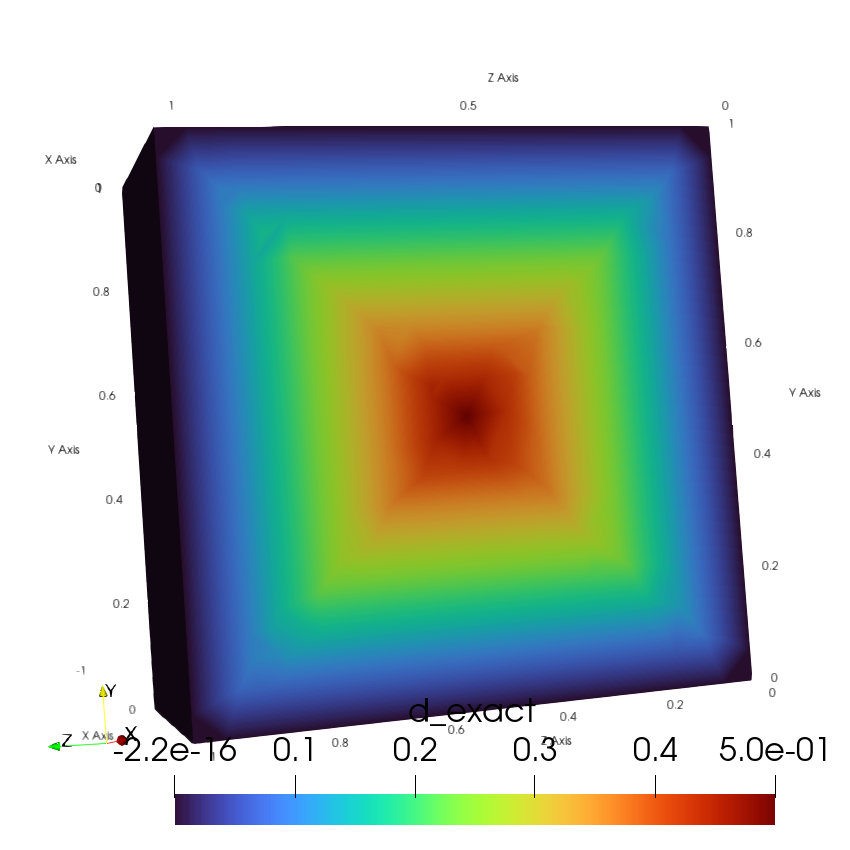
\includegraphics[width=\columnwidth]{graphics/feelpp/feelpp-benchmark-distance-exact}
        \caption{Exact distance $d_\mathrm{exact}$.}
        \label{fig:specs:app-feelpp-distance:results:distance}
    \end{subfigure}
    \begin{subfigure}{0.33\textwidth}
        \centering
        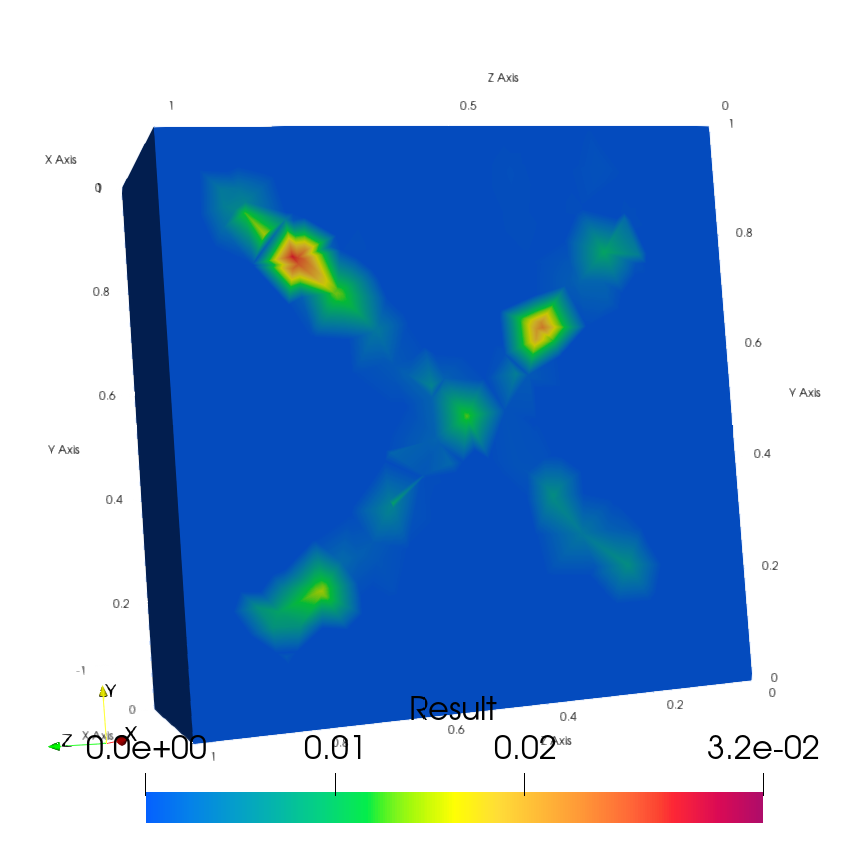
\includegraphics[width=\columnwidth]{graphics/feelpp/feelpp-benchmark-distance-errorFMM}
        \caption{Error by the method FMM: $|d_\mathrm{FMM}-d_\mathrm{exact}|$.}
        \label{fig:specs:app-feelpp-distance:results:error-fmm}
    \end{subfigure}
    \begin{subfigure}{0.33\textwidth}
        \centering
        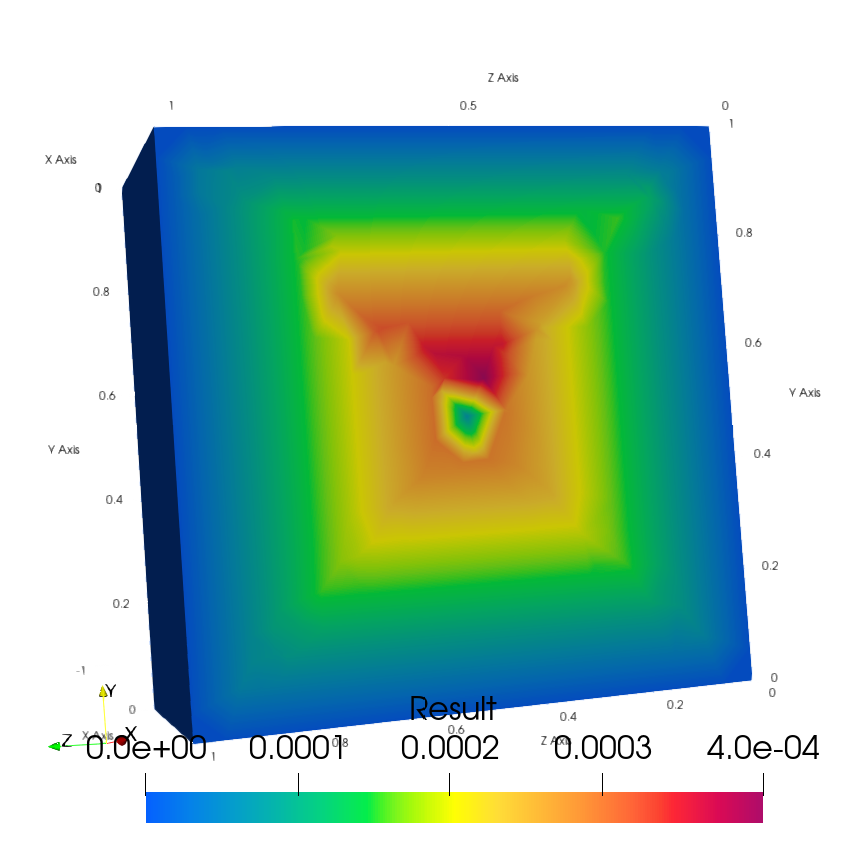
\includegraphics[width=\columnwidth]{graphics/feelpp/feelpp-benchmark-distance-errorBVH}
        \caption{Error by the method BVH: $|d_\mathrm{BVH}-d_\mathrm{exact}|$.}
        \label{fig:specs:app-feelpp-distance:results:error-bvh}
    \end{subfigure}
    \caption{Numerical results of distance computing, with $h=0.06$ and $M=1500$.}
    \label{fig:specs:app-feelpp-distance:results}
\end{figure}

We now present some results of convergence.

\pgfplotstableread[col sep=comma]{chapters/applications/specs/data/app-feelpp-distance/timeBVH1000.csv}\dataTimeBVHnp
\pgfplotstableread[col sep=comma]{chapters/applications/specs/data/app-feelpp-distance/speedupBVH1000.csv}\dataSpeedupBVHnp
\pgfplotstableread[col sep=comma]{chapters/applications/specs/data/app-feelpp-distance/timeFMM1000.csv}\dataTimeFMMnp
\pgfplotstableread[col sep=comma]{chapters/applications/specs/data/app-feelpp-distance/speedupFMM1000.csv}\dataSpeedupFMMnp
\pgfplotstableread[col sep=comma]{chapters/applications/specs/data/app-feelpp-distance/errorBVHRay.csv}\dataTimeBVHM
\pgfplotstableread[col sep=comma]{chapters/applications/specs/data/app-feelpp-distance/convergenceBVH.csv}\dataConvBVH
\pgfplotstableread[col sep=comma]{chapters/applications/specs/data/app-feelpp-distance/convergenceFMM.csv}\dataConvFMM


\begin{figure}
  \centering
  \begin{subfigure}{0.49\textwidth}
    \begin{tikzpicture}
    \begin{axis}[
      width=\textwidth,
      xlabel={ Number of tasks }, ylabel={ Time [s] },
      xtick=data, xtick align=outside,
      ymode=log,
      ymajorgrids=true, yminorgrids=true,
      xmajorgrids=true,
      xticklabels from table={\dataTimeBVHnp}{tasks},
      cycle list name=color list,
      legend style={ at={(0.5,1.05)}, anchor=south, legend columns=2 }
    ]
      \addplot+[mark=*, color=customorange] table [x expr=\coordindex, y=0.015] {\dataTimeBVHnp} ;
      \addlegendentry{ $h=0.015$ }
      \addplot+[mark=*, color=customcyan] table [x expr=\coordindex, y=0.03] {\dataTimeBVHnp} ;
      \addlegendentry{ $h=0.03$ }
      \addplot+[mark=*, dashed, color=customdarkblue] table [x expr=\coordindex, y=0.06] {\dataTimeBVHnp} ;
      \addlegendentry{ $h=0.06$ }
      \addplot+[mark=*, dashed, color=custompurple] table [x expr=\coordindex, y=0.12] {\dataTimeBVHnp} ;
      \addlegendentry{ $h=0.12$ }
    \end{axis}
    \end{tikzpicture}
      \caption{Evolution of the time for the BVH method depending on the number of parallel process, for various mesh sizes.}
    \label{fig:app:feelpp-distance:results:npBVH}
  \end{subfigure}
  \begin{subfigure}{0.49\textwidth}
    \begin{tikzpicture}
    \begin{axis}[
      width=\textwidth,
      xlabel={ Number of tasks }, ylabel={ Time [s] },
      xtick=data, xtick align=outside,
      ymode=log,
      ymajorgrids=true, yminorgrids=true,
      xmajorgrids=true,
      xticklabels from table={\dataSpeedupBVHnp}{tasks},
      cycle list name=color list,
      legend style={ at={(0.5,1.05)}, anchor=south, legend columns=2 }
    ]


      \addplot+[mark=*, color=customorange] table [x expr=\coordindex, y=0.015] {\dataSpeedupBVHnp} ;
      \addlegendentry{ $h=0.015$ }
      \addplot+[mark=*, color=customcyan] table [x expr=\coordindex, y=0.03] {\dataSpeedupBVHnp} ;
      \addlegendentry{ $h=0.03$ }
      \addplot+[mark=*, dashed, color=customdarkblue] table [x expr=\coordindex, y=0.06] {\dataSpeedupBVHnp} ;
      \addlegendentry{ $h=0.06$ }
      \addplot+[mark=*, dashed, color=custompurple] table [x expr=\coordindex, y=0.12] {\dataSpeedupBVHnp} ;
      \addlegendentry{ $h=0.12$ }
    \end{axis}
    \end{tikzpicture}
      \caption{Speedup of the BVH method, for various mesh sizes. }
    \label{fig:app:feelpp-distance:results:speedupBVH}
    \vspace{0.8\baselineskip}
  \end{subfigure}
  \caption{Time performance metrics for the BVH method of the mini-app distance}
\end{figure}




\begin{figure}
  \centering
  \begin{subfigure}{0.49\textwidth}
    \begin{tikzpicture}
    \begin{axis}[
      width=\textwidth,
      xlabel={ Number of tasks }, ylabel={ Time [s] },
      xtick=data, xtick align=outside,
      ymode=log,
      ymajorgrids=true, yminorgrids=true,
      xmajorgrids=true,
      xticklabels from table={\dataTimeFMMnp}{tasks},
      cycle list name=color list,
      legend style={ at={(0.5,1.05)}, anchor=south, legend columns=2 }
    ]
      \addplot+[mark=diamond*, color=customorange] table [x expr=\coordindex, y=0.015] {\dataTimeFMMnp} ;
      \addlegendentry{ $h=0.015$ }
      \addplot+[mark=diamond*, color=customcyan] table [x expr=\coordindex, y=0.03] {\dataTimeFMMnp} ;
      \addlegendentry{ $h=0.03$ }
      \addplot+[mark=diamond*, dashed, color=customdarkblue] table [x expr=\coordindex, y=0.06] {\dataTimeFMMnp} ;
      \addlegendentry{ $h=0.06$ }
      \addplot+[mark=diamond*, dashed, color=custompurple] table [x expr=\coordindex, y=0.12] {\dataTimeFMMnp} ;
      \addlegendentry{ $h=0.12$ }
    \end{axis}
    \end{tikzpicture}
      \caption{Evolution of the time for the FMM method depending on the number of parallel process, for various mesh sizes.}
    \label{fig:app:feelpp-distance:results:npFMM}
  \end{subfigure}
  \begin{subfigure}{0.49\textwidth}
    \begin{tikzpicture}
    \begin{axis}[
      width=\textwidth,
      xlabel={ Number of tasks }, ylabel={ Time [s] },
      xtick=data, xtick align=outside,
      ymode=log,
      ymajorgrids=true, yminorgrids=true,
      xmajorgrids=true,
      xticklabels from table={\dataSpeedupFMMnp}{tasks},
      cycle list name=color list,
      legend style={ at={(0.5,1.05)}, anchor=south, legend columns=2 }
    ]
      \addplot+[mark=diamond*, color=customorange] table [x expr=\coordindex, y=0.015] {\dataSpeedupFMMnp} ;
      \addlegendentry{ $h=0.015$ }
      \addplot+[mark=diamond*, color=customcyan] table [x expr=\coordindex, y=0.03] {\dataSpeedupFMMnp} ;
      \addlegendentry{ $h=0.03$ }
      \addplot+[mark=diamond*, dashed, color=customdarkblue] table [x expr=\coordindex, y=0.06] {\dataSpeedupFMMnp} ;
      \addlegendentry{ $h=0.06$ }
      \addplot+[mark=diamond*, dashed, color=custompurple] table [x expr=\coordindex, y=0.12] {\dataSpeedupFMMnp} ;
      \addlegendentry{ $h=0.12$ }
    \end{axis}
    \end{tikzpicture}
      \caption{Speedup of the FMM method, for various mesh sizes. }
    \label{fig:app:feelpp-distance:results:speedupFMM}
    \vspace{0.8\baselineskip}
  \end{subfigure}
  \caption{Time performance metrics for the FMM method of the mini-app distance}
\end{figure}

We show in \Cref{fig:app:feelpp-distance:results:npBVH,fig:app:feelpp-distance:results:npFMM} the evolution of the time taken by the two methods according to the number of parallel processes used.
The first result is that FMM takes less time than BVH, independently of the configuration.
It can also be noted that the execution time of the BVH method is almost independent of the number of parallel processes. A very small improvement can be observed for the $h=0.015$ case up to 8 cores, but then increases again.
The other meshes show an increase in execution time with the number of parallel processes.

Concerning the FMM method, it can be observed that the execution time decreases slightly with the number of parallel processes, but the speedup is not near optimal.


\begin{figure}
  \begin{subfigure}{0.49\textwidth}
    \begin{tikzpicture}
    \begin{axis}[
      width=\textwidth,
      xlabel={ Number of rays }, ylabel={ Error $L^2$ },
      xtick=data, xtick align=outside,
      ymode=log,
      ymajorgrids=true, yminorgrids=true,
      xmajorgrids=true,
      xticklabels from table={\dataTimeBVHM}{M},
      cycle list name=color list,
      legend style={ at={(0.5,1.05)}, anchor=south, legend columns=2 }
    ]
      \addplot+[mark=*, color=customdarkblue] table [x expr=\coordindex, y=0.12] {\dataTimeBVHM} ;
      \addlegendentry{ $h=0.12$ }
      \addplot+[mark=*, color=customcyan] table [x expr=\coordindex, y=0.06] {\dataTimeBVHM} ;
      \addlegendentry{ $h=0.06$ }
      \addplot+[mark=*, color=custompurple] table [x expr=\coordindex, y=0.03] {\dataTimeBVHM} ;
      \addlegendentry{ $h=0.03$ }
      \addplot+[mark=*, color=customorange] table [x expr=\coordindex, y=0.015] {\dataTimeBVHM} ;
      \addlegendentry{ $h=0.015$ }
    \end{axis}
    \end{tikzpicture}
    \caption{Evolution of the BVH error, regarding the number of rays cast.}
    \label{fig:app:feelpp-distance:results:M}
  \end{subfigure}%
  \hfill%
  \begin{subfigure}{0.49\textwidth}
    \begin{tikzpicture}
    \begin{axis}[
      width=\textwidth,
      xlabel={ $h$ }, ylabel={ Error $L^2$ },
      % xtick=data, xtick align=outside,
      ymode=log, xmode=log,
      ymin=3e-4,
      xmin=0.01, xmax=0.2,
      ymajorgrids=true, yminorgrids=true,
      xmajorgrids=true,
      % xticklabels from table={\dataConvBVH}{h},
      % cycle list name=color list,
      legend style={
        at={(0.99, 0.01)},
        nodes={scale=1, transform shape},
        anchor=south east
      }
    ]
      \addplot+[mark=*, color=customdarkblue, mark options={ fill=customdarkblue }, line width=1pt] table [x=h, y=100] {\dataConvBVH} ;
      \addlegendentry{ $M=100$ }
      \addplot+[mark=*, color=customcyan, mark options={ fill=customcyan }, line width=1pt] table [x=h, y=500] {\dataConvBVH} ;
      \addlegendentry{ $M=500$ }
      \addplot+[mark=*, color=customorange, mark options={ fill=customorange }, line width=1pt] table [x=h, y=1000] {\dataConvBVH} ;
      \addlegendentry{ $M=1000$ }
      \addplot+[mark=*, color=customgreen, mark options={ fill=customgreen }, line width=1pt] table [x=h, y=FMM] {\dataConvFMM} ;
      \addlegendentry{ FMM }

      \addplot+[color=black, dashed, mark=none, line width=1pt] table[x=h, y={create col/linear regression={y=1000}}]{\dataConvBVH};

    \end{axis}
    \end{tikzpicture}
    \caption{Convergence of the error against mesh size. The slope of the convergence is 1.5.}
    \label{fig:app:feelpp-distance:results:h}
  \end{subfigure}
  \caption{Metrics of results for the benchmark distance.}
  \label{fig:app:feelpp-distance:results}
\end{figure}

Now, we focus on the impact of the number of ray cast in the BVH method.
\Cref{fig:app:feelpp-distance:results:M} displays the evolution of the $L^2$ error depending on the number of ray $M$, for various sizes of mesh.
We see that the precision of the method for this specific benchmark is not impacted by this parameter, except for the finer mesh $h=0.015$ where the error decreases by a factor of ~2 between $M=100$ and $M=500$.

However, we can note that the impact of the mesh size is notably more important than the number of rays.

Precisely, we show in \Cref{fig:app:feelpp-distance:results:h} the convergence regarding the size of the discretization, we see a convergence at the order 1.5.
